\documentclass{../../../oss-apphys-exam}

\begin{document}
\genheader

\gentitle{C}{ELECTROSTATICS \& CAPACITORS}

\genmultidirections

\raggedcolumns
\begin{multicols*}{2}  
  \begin{questions}

    % THIS QUESTION IS TOO EASY; MOVE TO PHYSICS 2
%    \questions Two electric objects experience a repulsive force. What happens
%    to that force if the distance between the objects is doubled?
%    \begin{choices}
%      \choice It decreases to one-fourth its value.
%      \choice It decreases to one-half its value.
%      \choice It stays the same.
%      \choice It doubles.
%      \choice It quadruples.
%    \end{choices}
%    \vspace{.7in}

    % ALSO MOVE TO AP PHYSICS 2
%    \question A pith ball is a tiny piece of Styrofoam that is covered with a
%    conductive paint. One pith ball initially has a charge of \SI{6.4e-8}{C},
%    and it touches an identical, neutral pith ball. After the pith balls are
%    separated, what is the charge on the pith ball that had the initial charge?
%    \begin{choices}
%      \choice\SI{6.4e-8}{C}
%      \choice\SI{3.2e-8}{C}
%      \choice\SI{0}{C}
%      \choice\SI{-3.2e-8}{C}
%      \choice\SI{-6.4e-8}{C}
%    \end{choices}

    % ALSO MOVE TO AP PHYSICS 2
%    \question Glass becomes positively charged when it is rubbed with silk.
%    Which of the following is the best description of what’s happening?
%    \begin{choices}
%      \choice Electrons are rubbed off the glass onto the silk.
%      \choice Electrons are rubbed off the silk onto the glass.
%      \choice Protons are rubbed off the glass onto the silk.
%      \choice Protons are rubbed off the silk onto the glass.
%      \choice Neutrons in the glass have an affinity for positive charge.
%    \end{choices}

%    % ALSO MOVE TO AP PHYSICS 2
%    \question Consider an isolated, neutral system consisting of wool fabric
%    and a rubber rod. If the rubber rod is rubbed with wool to become negatively
%    charged, what can be said about the wool fabric?
%    \begin{choices}
%      \choice It becomes equally negatively charged.
%      \choice It becomes equally positively charged.
%      \choice It becomes negatively charged but not equally.
%      \choice It becomes positively charged but not equally.
%      \choice In a neutral system, neither object can become charged.
%    \end{choices}

    \question An electron and a proton are separated by \SI{1.50e-10}{\metre}.
    If they are released, which one will accelerate at a greater rate, and what
    is the magnitude of that acceleration?
    \begin{choices}
      \choice The electron; \SI{1.12e22}{m/s^2}
      \choice The proton; \SI{1.12e22}{m/s^2}
      \choice The electron; \SI{6.13e18}{m/s^2}
      \choice The proton; \SI{6.13e18}{m/s^2}
      \choice They both accelerate at the same rate; \SI{1.02e-8}{m/s^2}
    \end{choices}
   
    \question Four charges are arranged at the corners of a square of side a as
    shown. Which of the following is true of the electric field and the electric
    potential at the center of the square?
    \begin{center}
      \begin{tikzpicture}[scale=2]
        \draw[dashed](0,0)--(1,0)--(1,1) node[midway,right]{$a$}
        --(0,1)--cycle;
        \draw[fill=black](.5,.5) circle(0.03);
        \draw[fill=white](0,0) circle(.05) node[below left]{$-q$};
        \draw[fill=white](1,0) circle(.05) node[below right]{$+q$};
        \draw[fill=white](0,1) circle(.05) node[above left]{$+q$};
        \draw[fill=white](1,1) circle(.05) node[above right]{$-q$};
      \end{tikzpicture}
    \end{center}
    \begin{tabular}{rll}
      & \underline{Electric Field} & \underline{Electric Potential}\\
      (A) & zero & zero \\
      (B) & $\dfrac{kQ}{a\sqrt{2}}$ & zero \\
      (C) & $\dfrac{kQ^2}{2a^2}$ &  $\dfrac{kQ}{2a}$\\
      (D) & zero &  $\dfrac{kQ}{\sqrt{2a}}$\\
      (E) & $\dfrac{kQ^2}{2a}$ & $\dfrac{kQ}{a\sqrt{2}}$
    \end{tabular}
    \columnbreak
   
    \question Which of the following diagrams best represents how you might
    rearrange the charges so that the electric field at the center would point
    directly toward the top of the page?
   \begin{choices}
     \choice
     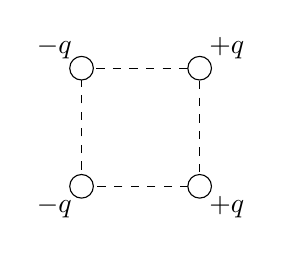
\begin{tikzpicture}[scale=1.5]
       \draw[dashed](0,0) rectangle(1,1);
       \draw[fill=white](0,0) circle(.1) node[below left]{$-q$};
       \draw[fill=white](1,0) circle(.1) node[below right]{$+q$};
       \draw[fill=white](0,1) circle(.1) node[above left]{$-q$};
       \draw[fill=white](1,1) circle(.1) node[above right]{$+q$};
     \end{tikzpicture}
     \choice
     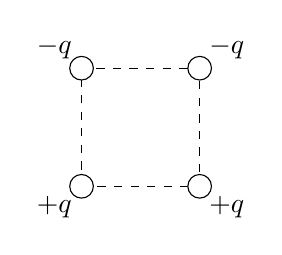
\begin{tikzpicture}[scale=1.5]
       \draw[dashed](0,0) rectangle(1,1);
       \draw[fill=white](0,0) circle(.1) node[below left]{$+q$};
       \draw[fill=white](1,0) circle(.1) node[below right]{$+q$};
       \draw[fill=white](0,1) circle(.1) node[above left]{$-q$};
       \draw[fill=white](1,1) circle(.1) node[above right]{$-q$};
     \end{tikzpicture}
     \choice
     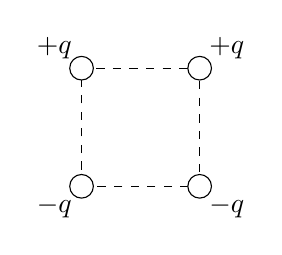
\begin{tikzpicture}[scale=1.5]
       \draw[dashed](0,0) rectangle(1,1);
       \draw[fill=white](0,0) circle(.1) node[below left]{$-q$};
       \draw[fill=white](1,0) circle(.1) node[below right]{$-q$};
       \draw[fill=white](0,1) circle(.1) node[above left]{$+q$};
       \draw[fill=white](1,1) circle(.1) node[above right]{$+q$};
     \end{tikzpicture}
     \choice
     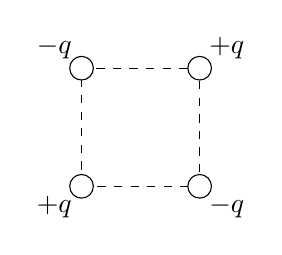
\begin{tikzpicture}[scale=1.5]
       \draw[dashed](0,0) rectangle(1,1);
       \draw[fill=white](0,0) circle(.1) node[below left]{$+q$};
       \draw[fill=white](1,0) circle(.1) node[below right]{$-q$};
       \draw[fill=white](0,1) circle(.1) node[above left]{$-q$};
       \draw[fill=white](1,1) circle(.1) node[above right]{$+q$};
     \end{tikzpicture}
     \choice
     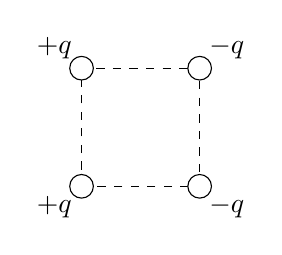
\begin{tikzpicture}[scale=1.5]
       \draw[dashed](0,0) rectangle(1,1);
       \draw[fill=white](0,0) circle(.1) node[below left]{$+q$};
       \draw[fill=white](1,0) circle(.1) node[below right]{$-q$};
       \draw[fill=white](0,1) circle(.1) node[above left]{$+q$};
       \draw[fill=white](1,1) circle(.1) node[above right]{$-q$};
     \end{tikzpicture}
   \end{choices}
   \columnbreak
   
   \question Three charges, $+Q$, $-Q$, and $+2Q$, are arranged in an
   equilateral triangle as shown. Which of the arrows below best represents the
   direction of the electric field at the center of the triangle?
   \begin{center}
     \vspace{-.1in}
     \begin{tikzpicture}[scale=2]
       \draw[dashed](0,0)--(1,0)--(.5,.866)--cycle;
       \draw (.5,.289) circle(.03);
       \draw[fill=white](0,0)     circle(.05) node[left] {$+Q\;$};
       \draw[fill=white](1,0)     circle(.05) node[right]{$\;-Q$};
       \draw[fill=white](.5,.866) circle(.05) node[above]{$2Q$};
     \end{tikzpicture}
   \end{center}
   \begin{choices}
     \choice {\Huge$\downarrow$}
     \choice {\Huge$\uparrow$}
     \choice {\Huge$\searrow$}
     \choice {\Huge$\swarrow$}
     \choice {\Huge$\nearrow$}
   \end{choices}
 
   \question A non-conducting sphere does not have a uniform charge density,
   but the density $\rho$ varies with the distance $r$ from the center of the
   sphere according to the equation $\rho=\beta r$ where $\beta$ is a positive
   constant. The electric field inside the sphere ($r<R$) at a distance $r$
   from the center of the sphere is
   \begin{choices}
     \choice $\dfrac{\beta r^2}{12\epsilon_0}$
     \choice $\dfrac{\beta r^3}{3\epsilon_0}$
     \choice $\dfrac{\beta r}{2\epsilon_0}$
     \choice $\dfrac{\beta r^2}{2\epsilon_0}$
     \choice $\dfrac{\beta r^2}{4\epsilon_0}$
   \end{choices}
 
   \question The electric potential at the surface of the sphere from the last
   question is
   \begin{choices}
     \choice $\dfrac{\beta R^3}{12\epsilon_0}$
     \choice $\dfrac{\beta R}{2\epsilon_0}$
     \choice $\dfrac{\beta R^3}{3\epsilon_0}$
     \choice $\dfrac{\beta R^2}{2\epsilon_0}$
     \choice $\dfrac{\beta R^2}{4\epsilon_0}$
   \end{choices}
   \columnbreak
   
   \question According to Gauss's law, the net electric flux passing through a
   closed surface is
   \begin{choices}
     \choice positive if the flux is entering the surface
     \choice negative if the flux is exiting the surface
     \choice positive if the net charge inside the surface is zero
     \choice negative if the net charge inside the surface is zero
     \choice zero if the net charge inside the surface is zero
   \end{choices}
   
   \question According to Gauss's law, which of the following statements is
   true?
   \begin{choices}
     \choice It is possible to have a nonzero electric field, but zero electric
     flux.
     \choice It is possible to have a nonzero electric flux, but zero electric
     field.
     \choice It is possible to have a nonzero electric flux through a closed
     surface even if the enclosed charge in a surface is zero.
     \choice If a surface is not closed (such as a sheet of paper), the flux
     through it must be zero.
     \choice It is possible for charges located outside a closed surface to
     produce a net positive flux through the surface.
   \end{choices}
   
   \question Electric potential
   \begin{choices}
     \choice is a vector quantity that depends on the direction of the electric
     field
     \choice is a scalar quantity that depends on the magnitude and sign of
     charges in the vicinity
     \choice is a scalar quantity that depends on the square of the distance
     from the charges in the vicinity
     \choice is a vector quantity that depends on the sign of the charges in the
     vicinity
     \choice is a vector quantity that must point from high to low potential
   \end{choices}
   \columnbreak
   
%   \question Gauss's law is most convenient to use when calculating an electric
%   field due to
%   \begin{choices}
%     \choice charges outside a closed surface
%     \choice charges inside a closed surface that has high symmetry
%     \choice charges inside a closed surface that has low symmetry
%     \choice a potential difference that is negative
%     \choice a potential difference that is positive
%   \end{choices}
%   \vspace{.7in}

   \question A positively charged ring of radius $R$ is made of conducting
   material and has a charge $Q$ distributed uniformly around it. The center of
   the ring is located at point $0$ on the $x$-axis. The potential $V$ at a
   distance $3d$ from point $0$ on the $x$-axis is
   \begin{center}
     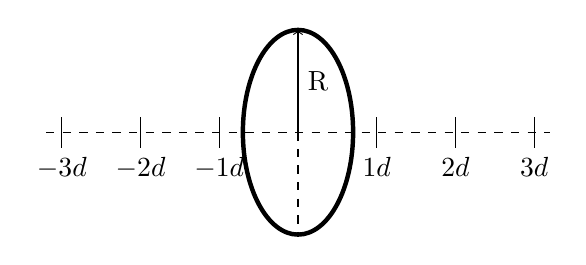
\begin{tikzpicture}
       \draw[ultra thick] (0,0) ellipse (0.7 and 1.3);
       \draw[->](0,0)--(0,1.3) node[midway,right]{R};
       \draw[dashed](0,0)--(0,-1.3);
       \draw[dashed](-3.2,0)--(3.2,0);
       \foreach \x in {-3,-2,-1,1,2,3}{
         \draw(\x,-.2)--(\x,.2) node[pos=0,below] {$\x d$};
       }
     \end{tikzpicture}
   \end{center}
   \begin{choices}
     \choice $V=\dfrac{kQ}{9d^2}$
     \choice $V=\dfrac{kQ}{3d^2}$
     \choice $V=\dfrac{kQ}{R^2+9d^2}$
     \choice $V=\sqrt{\dfrac{kQ}{R^2+9d^2}}$
     \choice $V=\dfrac{kQ}{\sqrt{R^2+9d^2}}$
   \end{choices}
   
   \uplevel{
     \textbf{Question \ref{cube1}-\ref{cube2}}
     \cpic{.35}{cube}
   }
   \question A cube has sides of length $a$. The cube rests so that one side
   rests on the $x$-axis as shown. An electric field is established in the
   $x$-direction according to the function $E_x=bx^2$ , where $b$ is a positive
   constant. Which of the following statements is true?
   \label{cube1}
   \begin{choices}
     \choice There is a net charge inside the cube.
     \choice There is no net charge inside the cube.
     \choice The flux passing through the cube is negative.
     \choice The flux passing through the cube is zero.
     \choice The flux diminishes while passing through the cube.
   \end{choices}
   \columnbreak
   
   \question The charge inside the cube can be expressed by the equation
   \label{cube2}
   \begin{choices}
     \choice $\epsilon_0ba$
     \choice $\epsilon_0ba^2$
     \choice $\epsilon_0ba^3$
     \choice $\epsilon_0ba^4$
     \choice $\epsilon_0b^22a^2$
   \end{choices}
   
   \question Which of the following statements is true of electric field and
   equipotential lines?
   \begin{choices}
     \choice The electric field vector always points in the same direction as
     the equipotential lines.
     \choice The electric field always points in the opposite direction of the
     equipotential lines.
     \choice The electric field always points perpendicular to the equipotential
     lines.
     \choice The electric field is always equal to the equipotential lines.
     \choice Equipotential lines always form a circle around electric field
     lines.
   \end{choices}
   
   \question The potential $V$ as a function of distance $r$ for a particular
   charge distribution is given by the equation $V=ar^{-1}$. The electric field
   as a function of distance $r$ from the charge distribution is
   \begin{choices}
     \choice $\dfrac13ar^{-3}$
     \choice $2ar^{-1}$
     \choice $ar^{-2}$
     \choice $-a(\ln r)$
     \choice $-ar^{-2}$
   \end{choices}
   \columnbreak
   
%  \vspace{-0.5in}
%  \begin{center}
%    \begin{tikzpicture}[scale=0.7]
%      \draw[fill=gray!60](0,0) circle(0.25);
%      \draw[dashed](0,0) circle(1);
%      \draw[dashed](0,0) circle(3);
%      \draw(0,0)--(1,0) node[pos=1,right]{$x$} node[midway,above]{$R$};
%      \draw[fill=black](1,0) circle(0.05);
%      \begin{scope}[rotate=230]
%        \draw(0,0)--(3,0) node[pos=1,right]{$y$} node[pos=0.7,right]{$3R$};
%        \draw[fill=black](3,0) circle(0.05);
%      \end{scope}
%    \end{tikzpicture}
%   %  \end{center}

   \uplevel{
     \textbf{Questions \ref{cap1}--\ref{cap2}}
     \begin{center}
       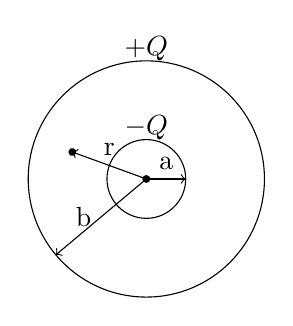
\begin{tikzpicture}[scale=.5]
         \draw(0,0) circle(1);
         \draw(0,0) circle(3);
         \fill(0,0) circle(.1);
         \draw[->](0,0)--(1,0) node[midway,above]{a};
         \draw[->,rotate=-140](0,0)--(3,0) node[midway,left]{b};
         \begin{scope}[rotate=160]
           \draw[->](0,0)--(2,0) node[midway,above]{r};
           \fill(2,0) circle(.1);
         \end{scope}
         \node at (0,3.3) (a){$+Q$};
         \node at (0,1.3) (b){$-Q$};
       \end{tikzpicture}
     \end{center}
     The spherical capacitor shown above consists of a conducting shell of
     radius $a$ inside a larger conducting shell of radius $b$. A charge $-Q$
     is placed on the inner sphere and a charge $+Q$ is placed on the outer
     shell. The capacitance of the capacitor is $C_0$.
   }
   \question The magnitude of the electric field $E$ at a distance $r$ between
   the spheres is
   \label{cap1}
   \begin{choices}
     \choice $\dfrac{Q}{4\pi\epsilon_0r^2}$
     \choice $\dfrac{Q}{4\pi\epsilon_0r}$
     \choice $\dfrac{Q}{4\pi\epsilon_0a^2}$
     \choice $\dfrac{Q}{4\pi\epsilon_0b^2}$
     \choice zero
   \end{choices}

   \question The bottom half of the space between the spheres is filled with
   oil of dielectric constant $\kappa=3$, creating two capacitors connected to
   each other. Which of the following is true of the two capacitors?
    \begin{center}
      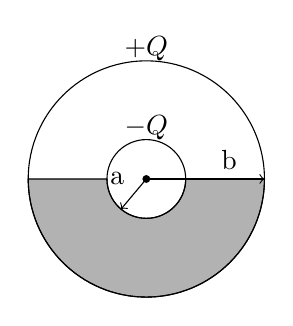
\begin{tikzpicture}[scale=.5]
        \draw[fill=gray!60](-1,0)--(-3,0) arc(180:360:3)--(1,0) arc(0:-180:1);
        \draw(0,0) circle(1);
        \draw(0,0) circle(3);
        \fill(0,0) circle(.1);
        \draw[->,rotate=230](0,0)--(1,0) node[midway,above left]{a};
        \draw[->](0,0)--(3,0) node[pos=.7,above]{b};
        \node at (0,3.3) (a){$+Q$};
        \node at (0,1.3) (b){$-Q$};
      \end{tikzpicture}
    \end{center}
    \begin{choices}
      \choice They are connected in series.
      \choice They are connected in parallel.
      \choice The total capacitance has not changed.
      \choice The total capacitance of the spheres has decreased.
      \choice The total capacitance is now zero.
    \end{choices}
    
    \question With the bottom half of the space between the spheres having been
    filled with oil of dielectric constant $\kappa=3$, the new capacitance of
    the spheres is
    \label{cap2}
    \begin{choices}
      \choice zero
      \choice $C_0$
      \choice $2C_0$
      \choice $3C_0$
      \choice $4C_0$
    \end{choices}   
  \end{questions}
\end{multicols*}
\newpage

\genfreetitle{C}{ELECTROSTATICS \& CAPACITORS}{6}

\genfreedirections

% TAKEN FROM 2007 AP PHYSICS C EXAM FREE-RESPONSE QUESTION E&M 2
\cpic{.3}{charges}
\begin{questions}
  \question In the figure above, a nonconducting solid sphere of radius a with
  charge $+Q$ uniformly distributed throughout its volume is concentric with a
  nonconducting spherical shell of inner radius $2a$ and outer radius $3a$ that
  has a charge $-Q$ uniformly distributed throughout its volume. Express all
  answers in terms of the given quantities and fundamental constants.

  \begin{parts}
    \part Using Gauss's law, derive expressions for the magnitude of the
    electric field as a function of radius $r$ in the following regions.
    \begin{subparts}
      \subpart Within the solid sphere ($r<a$)
      \subpart Between the solid sphere and the spherical shell ($a<r<2a$)
      \subpart Within the spherical shell ($2a<r<3a$)
      \subpart Outside the spherical shell ($r>3a$)
    \end{subparts}
    
    \part What is the electric potential at the outer surface of the spherical
    shell ($r=3a$)? Explain your reasoning.
    
    \part Derive an expression for the electric potential difference $V_X-V_Y$
    between points $X$ and $Y$ shown in the figure.
  \end{parts}
  \newpage

  % TAKEN FROM 2010 AP PHYSICS C EXAM FREE-RESPONSE QUESTION E&M 1
  \uplevel{
    \cpic{.28}{circle}
  }
  \question A charge $+Q$ is uniformly distributed over a quarter circle of
  radius $R$, as shown above. Points $A$, $B$, and $C$ are located as shown,
  with $A$ and $C$ located symmetrically relative to the $x$-axis. Express all
  algebraic answers in terms of the given quantities and fundamental constants.
  \begin{parts}
    \part Rank the magnitude of the electric potential at points $A$, $B$, and
    $C$ from greatest to least, with number 1 being greatest. If two points have
    the same potential, give them the same ranking. Justify your rankings.

    \vspace{.1in}
    \underline{\hspace{.3in} } $V_A$ \hspace{.3in}
    \underline{\hspace{.3in} } $V_B$ \hspace{.3in}
    \underline{\hspace{.3in} } $V_C$
    
    \uplevel{
      Point $P$ is at the origin, as shown below, and is the center of curvature
      of the charge distribution.
      \cpic{.28}{circle2}
    }

    \part Determine an expression for the electric potential at point $P$ due to
    the charge $Q$.

    \part A positive point charge $q$ with mass $m$ is placed at point $P$ and
    released from rest. Derive an expression for the speed of the point charge
    when it is very far from the origin.    

    \part On the dot representing point $P$ below, indicate the direction of the
    electric field at point P due to the charge $Q$.
    \begin{center}
      \begin{tikzpicture}[scale=1.2]
        \draw[dashed,->](-1,0)--(1,0) node[right]{$x$};
        \draw[dashed,->](0,-1)--(0,1) node[above]{$y$};
        \fill(0,0) circle(.1);
      \end{tikzpicture}
    \end{center}
    
    \part Derive an expression for the magnitude of the electric field at point
    $P$.
  \end{parts}
  \newpage
  
%\item In the Bohr model of the hydrogen atom, the electron moves in a circular
%  orbit of radius $r$ around the proton.
%  \begin{enumerate}
%  \item Find an expression for the kinetic energy of the electron as a function
%    of $r$. Show that at any distance $r$ the kinetic energy is half the
%    potential energy.
%  \item Evaluate kinetic energy $K$, potential energy $U$ and the total
%    energy $W=K+U$ in electron volts for\\ $r=\SI{0.529e-10}{\metre}$, the
%    radius of the electron's orbit in hydrogen. (The energy $|W|$ that must be
%    supplied to the hydrogen atom to remove the electron is called the
%    ionization energy.)
%  \end{enumerate}
%  \newpage

  % TAKEN FROM 2016 AP PHYSICS C EXAM FREE-RESPONSE QUESTION E&M 1
  \uplevel{
    \cpic{.9}{potentials}
  }
  \question Two point charges, $q_1$ and $q_2$, are fixed in place on the
  $x$-axis at positions $x_1=\SI{-1.00}{\metre}$ and $x_1=+\SI{0.50}{\metre}$,
  respectively. Charge $q_2$ has a value of $+2.0$ nC. Values of electric
  potential are illustrated by the given equipotentials in the diagram shown
  above, which is drawn to scale.
  \begin{parts}
    \part Calculate the value of $q_1$.
    
    \part At point $C$ on the diagram, draw a vector representing the direction
    of the electric field at that point.
    
    \part Calculate the approximate magnitude of the electric field strength at
    point $D$ on the diagram.
    
    \part The equipotential labeled $\SI{0}{\volt}$ is the cross section of a
    nearly spherical surface. Calculate the electric flux for this surface.
    
    \part A proton is placed at point $A$ and then released from rest.
    \begin{subparts}
      \subpart Calculate the work done by the electric field on the proton as it
      moves from point $A$ to point $E$.
      
      \subpart Calculate the speed of the proton when it reaches point $E$.
    \end{subparts}
    
    \part An electron is released from rest at point $B$. Which of the following
    indicates the direction of the initial acceleration, if any, of the
    electron? Justify your answer.

    \vspace{.1in}
    \underline{\hspace{.3in}} Up\hspace{.2in}
    \underline{\hspace{.3in}} Down\hspace{.2in}
    \underline{\hspace{.3in}} Left\hspace{.2in}
    \underline{\hspace{.3in}} Right\hspace{.2in}
    \underline{\hspace{.3in}} Into the page\hspace{.2in}
    \underline{\hspace{.3in}} Out of the page

    \vspace{.1in}\underline{\hspace{.3in}} The direction is undefined since the
    acceleration is zero.
  \end{parts}
  \newpage

  % TAKEN FROM 2003 AP PHYSICS C EXAM FREE-RESPONSE QUESTION E&M 1. THE
  % TIKZ FIGURE BELOW IS A FAIRLY GOOD REPRODUCTION OF THE ORIGINAL AP EXAM
  % DIAGRAM.
  \uplevel{
    \centering
    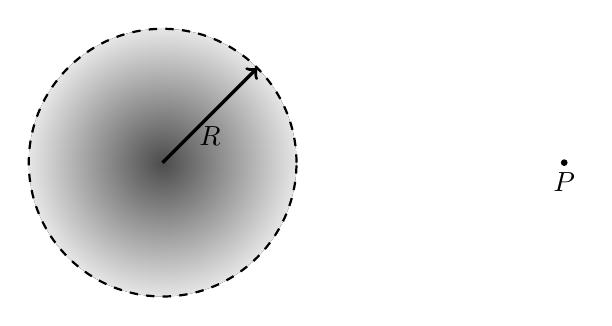
\begin{tikzpicture}[scale=.85]
      \filldraw[dashed,thick,
        even odd rule,
        inner color=black!70,
        outer color=gray!20] (0,0) circle (2);
      \draw[very thick,->,rotate=45](0,0)--(2,0) node[midway,below]{$R$};
      \fill(6,0) circle(.05) node[below]{$P$};
    \end{tikzpicture}
  }
  \question A spherical cloud of charge of radius $R$ contains a total charge
  $+Q$ with a nonuniform volume charge density that varies according to the
  equation
  \begin{align*}
    \rho(r)&= \rho_0\left( 1 -\dfrac rR \right)\text{ for }r\leq R\text{ and}\\
    \rho(r)&= 0\text{ for }r>R
  \end{align*}
  where $r$ is the distance from the center of the cloud. Express all algebraic
  answers in terms of $Q$, $R$, and fundamental constants.
  \begin{parts}
    \part Determine the following as a function of $r$ for $r>R$.
    \begin{subparts}
      \subpart The magnitude $E$ of the electric field
      \subpart The electric potential $V$
    \end{subparts}
    \part A proton is placed at point $P$ shown above and released. Describe its
    motion for a long time after its release.
    
    \part An electron of charge magnitude $e$ is now placed at point $P$, which
    is a distance $r$ from the center of the sphere, and released. Determine
    the kinetic energy of the electron as a function of $r$ as it strikes the
    cloud.
    
    \part Derive an expression for $\rho_0$.
    
    \part Determine the magnitude $E$ of the electric field as a function of $r$
    for $r\leq R$.
  \end{parts}
  \newpage

  % TAKEN FROM THE 2004 AP PHYSICS C FREE-RESPONSE QUESTION E&M 1. NO CHANGES TO
  % THE QUESTION HAVE BEEN MADE
  \uplevel{
    \cpic{.65}{nonconcentric}
  }
  \question The figure above left shows a hollow, infinite, cylindrical,
  uncharged conducting shell of inner radius $r_1$ and outer radius $r_2$. An
  infinite line charge of linear charge density $+\lambda$ is parallel to its
  axis but off center. An enlarged cross section of the cylindrical shell is
  shown above right.
  \begin{parts}
    \part On the cross section above right,
    \begin{subparts}
      \subpart sketch the electric field lines, if any, in each of regions I,
      II, and III and
      \subpart use $+$ and $-$ signs to indicate any charge induced on the
      conductor.
      \end{subparts}
    \part In the spaces below, rank the electric potentials at points $a$, $b$,
    $c$, $d$, and $e$ from highest to lowest (1 = highest potential). If two
    points are at the same potential, give them the same number.

    \vspace{.1in}
    \underline{\hspace{.2in}} $V_a$\hspace{.3in}
    \underline{\hspace{.2in}} $V_b$\hspace{.3in}
    \underline{\hspace{.2in}} $V_c$\hspace{.3in}
    \underline{\hspace{.2in}} $V_d$\hspace{.3in}
    \underline{\hspace{.2in}} $V_e$
    \uplevel{
      \cpic{.65}{concentric}
    }

    \part The shell is replaced by another cylindrical shell that has the same
    dimensions but is nonconducting and carries a uniform volume charge density
    $+\rho$. The infinite line charge, still of charge density $+\lambda$, is
    located at the center of the shell as shown above. Using Gauss's law,
    calculate the magnitude of the electric field as a function of the distance
    $r$ from the center of the shell for each of the following regions. Express
    your answers in terms of the given quantities and fundamental constants.
    \begin{subparts}
      \subpart $r < r_1$
      \subpart $r_1\leq r\leq r_2$
      \subpart $r > r_2$
    \end{subparts}
  \end{parts}
  \newpage
    
  \question A spherically symmetric charge distribution has net positive charge
  $Q_0$ distributed within a radius of $R$. Its electric potential $V$ as a
  function of the distance $r$ from the center of the sphere is given by the
  following
  \begin{align*}
    V(r) &= \frac{Q_0}{4\pi\epsilon_0R}\left[-2+3\left(\frac rR\right)^2 \right]
    \text{ for } r<R\\
    V(r) &= \frac{Q_0}{4\pi\epsilon_0r}\text{ for } r>R
  \end{align*}
  Express all algebraic answers in terms of the given quantities and
  fundamental constants.
  \begin{parts}
    \part For the following regions, indicate the direction of the electric
    field $E(r)$ and derive an expression for its magnitude.
    \begin{subparts}
      \subpart $r < R$
      
      \vspace{.1in}\underline{\hspace{.4in}} Radially inward
        
      \vspace{.1in}\underline{\hspace{.4in}} Radially outward
      
      \subpart $r > R$
      
      \vspace{.1in}\underline{\hspace{.4in}} Radially inward

      \vspace{.1in}\underline{\hspace{.4in}} Radially outward
    \end{subparts}
    
    \part For the following regions, derive an expression for the enclosed
    charge that generates the electric field in that region, expressed as a
    function of $r$.
    \begin{subparts}
      \subpart $r < R$
      \subpart $r > R$
    \end{subparts}

    \part Is there any charge on the surface of the sphere ($r=R$)?

    \vspace{.1in}
    \underline{\hspace{.4in}} Yes\hspace{.3in}
    \underline{\hspace{.4in}} No
    
    If there is, determine the charge. In either case, explain your reasoning.

    \part On the axes below, sketch a graph of the force that would act on a
    positive test charge in the regions $r<R$ and $r > R$. Assume that a force
    directed radially outward is positive.
    \begin{center}
      \begin{tikzpicture}[scale=1.1]
        \draw[very thick,->](0,-3)--(0,3) node[above]{$F$};
        \draw[very thick,->](0,0)--(10,0) node[right]{$r$};
        \draw[dashed](4,-3)--(4,3) node[midway,below left]{$R$};
      \end{tikzpicture}
    \end{center}
  \end{parts}
  \newpage


  
%\item Two identical small spheres of mass $m$ are suspended from a common point
%  by threads of length $L$. When each sphere carries a charge $q$, each thread
%  makes an angle $\theta$ with the vertical as shown in the figure below.
%  \begin{enumerate}
%  \item Express charge $q$ in terms of $\theta$, $m$, $L$ and any other relevant
%    constants, and
%  \item Compute $q$ if $m=\SI{10}{\gram}$, $L=\SI{50}{\centi\metre}$ and
%    $\theta=\ang{10}$.
%  \end{enumerate}
%  \begin{tikzpicture}[scale=1.3]
%    \tikzstyle{balloon}=[ball color=red!60];
%    \fill[yellow!85!gray](-1.5,0) rectangle(1.5,0.15);
%    \draw[very thick,yellow](-1.5,0)--(1.5,0);
%    \draw[dashed,very thick,blue!80!gray](0,0)--(0,-4);
%    \draw[<->](0,-2.5) arc (270:285:2.5) node[midway,below]{$\theta$};
%    \draw[<->](0,-2.5) arc (270:255:2.5) node[midway,below]{$\theta$};
%    \begin{scope}[rotate=15]
%      \draw(0,0)--(0,-3.5) node[midway,right]{$L$};
%      \shade[balloon] (0,-3.5) circle (0.25) node[below]{$q$};
%    \end{scope}
%    \begin{scope}[rotate=-15]
%      \draw(0,0)--(0,-3.5) node[midway,left]{$L$};
%      \shade[balloon] (0,-3.5) circle (.25) node[below]{$q$};
%    \end{scope}
%  \end{tikzpicture}
%  \vspace{\stretch{1}}
   
%\item Five equal charges $Q$ are equally spaced on a semicircle or radius $R$
%  as shown in the figure below. Find the force on a charge $q$ located at the
%  center of the semi-circle. (Hint: Take advantage of symmetry.)
%  
%  \begin{tikzpicture}[scale=1.2]
%    \tikzstyle{balloon}=[ball color=yellow!40];
%    \draw(0,-1.75)--(0,3) node[pos=1,above]{$y$};
%    \draw(0,0)--(2.75,0) node[pos=1,right]{$x$};
%    \draw[->,rotate=120](0,0)--(1.75,0) node[midway,above right]{$R$};
%    \draw(0,1.75) arc (90:270:1.75);
%    \foreach \x in {0,45,...,180}
%    \shade[balloon,rotate=\x] (0,1.75) circle (0.2) node[left]{$Q\;\;$};
%    \shade[balloon] (0,0) circle(0.12) node[right]{$\;q$};
%  \end{tikzpicture}
%  \vspace{\stretch{1}}
%  \newpage
  
%\item Two positive charges $+q$ are on the $y$ axis at $y=+a$ and $y=-a$.
%  \begin{enumerate}
%  \item Show that the electric field on the $x$ axis is along the $x$ axis with
%    $E_x=2kqx(x^2+a^2)^{-3/2}$.
%  \item Show that near the origin, when $x\ll a$, $E_x\approx 2kqx/a^3$.
%  \item Show that for $x\gg a$, $E_x\approx 2kq/x^2$.
%  \item Explain why you should expect the result in (c) even before calculating
%    it.
%  \end{enumerate}
%  A bead of mass $m$ with a negative charge $-q$ slides along a thread that
%  runs along the $x$ axis.
%  \begin{enumerate}[resume]
%  \item Show that for small displacements $x\ll a$, the bead experiences a
%    restoring force that is proportional to $x$ and therefore undergoes
%    simple harmonic motion.
%  \item Find the period of the motion.
%  \end{enumerate}
%  %\vspace{\stretch{4}}
%  \newpage
  
%\item Using Gauss's law, find
%  \begin{enumerate}
%  \item the electric field strength inside and outside of a uniformly charged
%    hollow sphere of radius $R$ and surface charge density $\sigma$ (charge
%    per unit area).
%  \item the electric field inside and outside an infinitely long cyclindrical
%    shell of charge of radius $R$ with charge discibution $\sigma$ (charge
%    per unit area).
%  \item the electric field strength inside and outside a infinitely long solid
%    cylinder of radius $R$ carrying a linear uniform charge density $\rho$
%    (charge per unit volume).
%  \end{enumerate}
%  Hint: In all cases, think about where to put the Gaussian surface. Take
%  advantage of symmetry.
%  %\vspace{\stretch{1}}
%  \newpage

%\item For the circuit shown below, find
%  \begin{enumerate}[noitemsep]
%  \item The total equivalent capacitance between the terminals
%  \item The charge stored on each capacitor
%  \item the total stored charge
%  \end{enumerate}
%  \begin{tikzpicture}[scale=1.2,american voltages]
%    \draw[thick] (0,2) to[C=0.30<\micro\farad>,*-] (3,2)
%    to[C=1.0<\micro\farad>] (3,0) to[short,-*](0,0);
%    \draw[thick] (3,2)--(5,2) to[C=0.25<\micro\farad>,] (5,0)--(3,0);
%  \end{tikzpicture}
%  \vspace{\stretch{1}}
  
%\item A parallel-plate capacitor has a capacitance $C_0$ and plate separation
%  of $d$. To dielectric slabs of constants $\kappa_1$ and $\kappa_2$, each of
%  thickness $d/2$ and having the same area as the plates, are inserted between
%  the plates as shown in the figure below. When the free charge on the plates
%  are $Q$,
%  \begin{enumerate}
%  \item find the electric field in each of the dielectric
%  \item find the potential difference between the plates
%  \item show that the new capacitance is given by:
%    $\displaystyle C=\frac{\kappa_1\kappa_2}{\kappa_1+\kappa_2}C_0$
%  \end{enumerate}
%  \pic{.2}{stacked}
%  %\vspace{\stretch{1}}

%\item Several point charges produce the equipotential lines shown.
%  \begin{enumerate}[noitemsep]
%  \item At which point on the diagram is the magnitude of the electric field
%    greatest? Explain.
%  \item Points C and D are approximately \SI{.02}{\metre} apart. Point F is
%    halfway between points C and D. What is the electric field at point F?
%  \item A \SI{5.}{\micro\coulomb} point charge is moved from point C to point
%    E, then to point D by an external force. Determine the work done by the
%    external force.
%  \end{enumerate}
%  \pic{.45}{equipotentials}
%  \vspace{\stretch{1}}

%\item A potential is given by
%  \begin{displaymath}
%    V(x,y,z)=\frac{kQ}{\sqrt{(x-a)^2+y^2+z^2}}
%  \end{displaymath}
%  \begin{enumerate}[noitemsep]
%  \item Find the components $E_x$, $E_y$ and $E_z$ of the electric field by
%    differentiating this potential function.
%  \item What simple charge distribution might be responsible for this potential?
%  \end{enumerate}
%  \vspace{\stretch{1}}
\end{questions}
\end{document}
